\documentclass{article}

\usepackage[T1]{fontenc}
\usepackage[utf8]{inputenc}
\usepackage{lmodern}
\usepackage{listings}
\usepackage[colorlinks = true,
            linkcolor = blue,
            urlcolor  = blue,
            citecolor = blue,
            anchorcolor = blue]{hyperref}
\usepackage{graphicx}
\usepackage{subfig}
\usepackage[dvipsnames,table,xcdraw]{xcolor}
\usepackage{array}
\newcolumntype{P}[1]{>{\centering\arraybackslash}p{#1}}
\newcolumntype{M}[1]{>{\centering\arraybackslash}m{#1}}
\author{Francesco Boi}
\title{Self-driving cars program - project  2: Advanced Lane Detection}
\date{}

\let\cd\lstinline

\begin{document}
% Python style for highlighting

\maketitle
\tableofcontents 

\lstdefinestyle{customc}{
  belowcaptionskip=1\baselineskip,
  breaklines=true,
  %frame=L,
  xleftmargin=\parindent,
  language = Python,
  showstringspaces=false,
  basicstyle=\footnotesize\ttfamily,
  keywordstyle=\bfseries\color{blue!85!black},
  commentstyle=\itshape\color{gray},
  identifierstyle=\color{black},
  stringstyle=\color{red},
  numbers=left,                    				% where to put the line-numbers; possible values are (none, left, right)
  numbersep=5pt,                   			% how far the line-numbers are from the code
  numberstyle=\tiny\color{gray},     % the style that is used for the line-numbers
  stepnumber=1,
  tabsize=4,
}
\lstdefinestyle{customasm}{
  belowcaptionskip=1\baselineskip,
  frame=L,
  %xleftmargin=\parindent,
  language=[x86masm]Assembler,
  basicstyle=\footnotesize\ttfamily,
  commentstyle=\itshape\color{purple!40!black},
  stepnumber=1,
   tabsize=4,
}
\definecolor{lightgray}{rgb}{.9,.9,.9}
\definecolor{darkgray}{rgb}{.4,.4,.4}
\definecolor{purple}{rgb}{0.65, 0.12, 0.82}
\lstset{escapechar=ç,style=customc}
\section{Content of the project}
Here is the content of the project:
\begin{itemize}
\item \textit{writeup.pdf} (this file): report of the project;
\item \textit{camera\_cal}: folder containing the images to be used for camera calibration;
\item \textit{P2.ipynb}: ipython notebook with the code for advanced lane detection;
\item \textit{test\_images}: folder containing the images to be used as tests;
\item \textit{output\_images}: folder containing a subfolder for each image in \textit{test\_images}; each subfolder contains the resulting images for every step of the pipeline;
\item \textit{project\_video.mp4}: input video of the project
\item \textit{challenge\_video.mp4}: additional video;
\item \textit{harder\_challenge\_video.mp4}: additional video;
\item \textit{output}: folder containing the annotated videos resulting from the pipeline and matrices to undistort, warp and unwarp the images;
\end{itemize}

\section{Project goals}
The steps of this project are the following:
\begin{itemize}
\item Compute the camera calibration matrix and distortion coefficients given a set of chessboard images. Apply a distortion correction to raw images.
\item Use color transforms, gradients, etc., to create a thresholded binary image.
\item Apply a perspective transform to rectify binary image ("birds-eye view").
\item Detect lane pixels and fit to find the lane boundary.
\item Determine the curvature of the lane and vehicle position with respect to center.
\item Warp the detected lane boundaries back onto the original image.
\item Output visual display of the lane boundaries and numerical estimation of lane curvature and vehicle position.
\end{itemize}

\section{Camera calibration}
Camera calibration is performed from cell 7 to 10 of the jupyter notebook, in the section \textit{Camera calibration}. The assumption is that the chessboard lies on the plane with $z=0$, hence the object points are the same for each calibration image. 

Cell 8 (executed cell 6) prepares \cd+objp+, a list containing $(x, y, z)$ coordinates of the chessboard corners in the world for a single image. Since \cd+objp+ is the same for every calibration image, a copy of it will be appended  every time chessboard corners are successfully detected in a test image.
\cd+imgpoints+ will be appended with the $(x, y)$ pixel position of each of the corners in the image plane with each successful chessboard detection. 

In cell 10 (executed cell 7) \cd+objpoints+ and \cd+imgpoints+ are used to compute the camera calibration and distortion coefficients using the \cd+cv2.calibrateCamera()+ function. Relevant matrices are saved in the pickle file \cd+output/wide_dist_pickle.p+ as dictionary.

Once the matrix has been calculated, the image can be corrected with the function \cd+cv2.undistort(image, mtx, dist, None, mtx)+. Results of the distortion correction are shown in the folder \cd+output_images/+ \cd+calibration_result+; an example is shown in \autoref{fig:distCorr}.

\begin{figure}
\subfloat[Original image.]{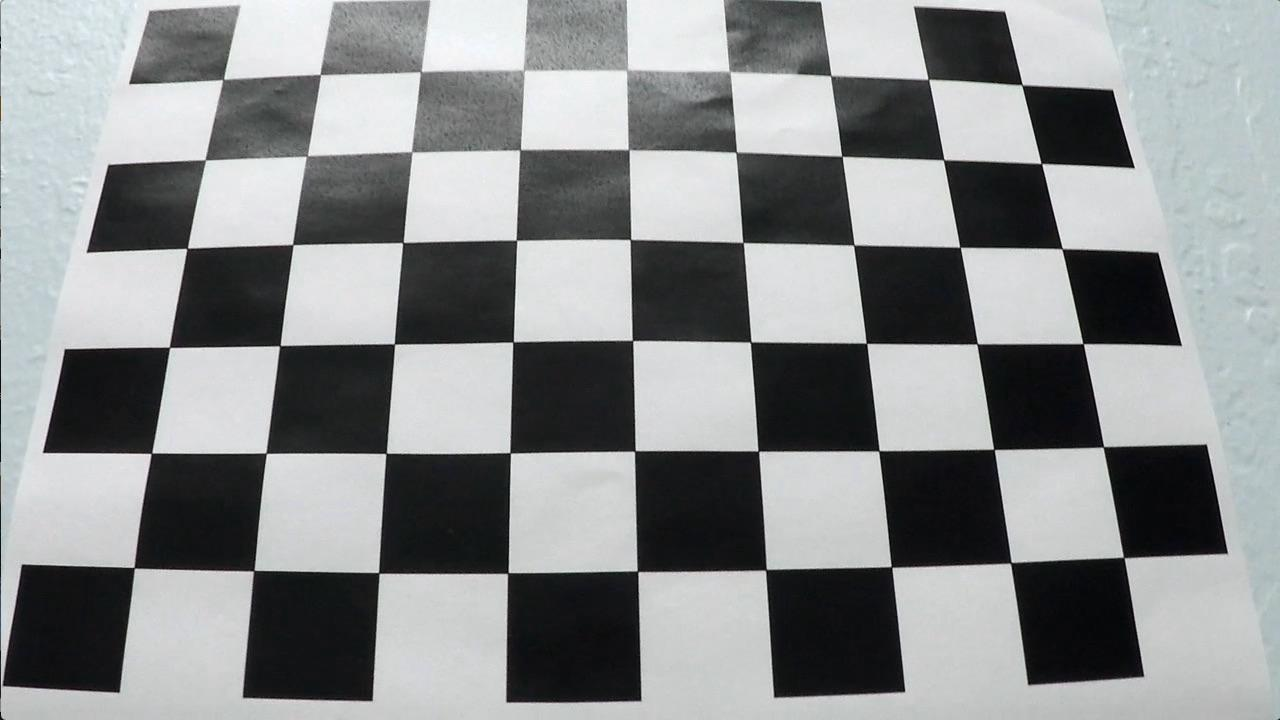
\includegraphics[width=0.5\textwidth]{output_images/calibration_result/calibration3/original.jpg}\label{fig:distCorrf1}}
\hfill
\subfloat[Undistorted image.]{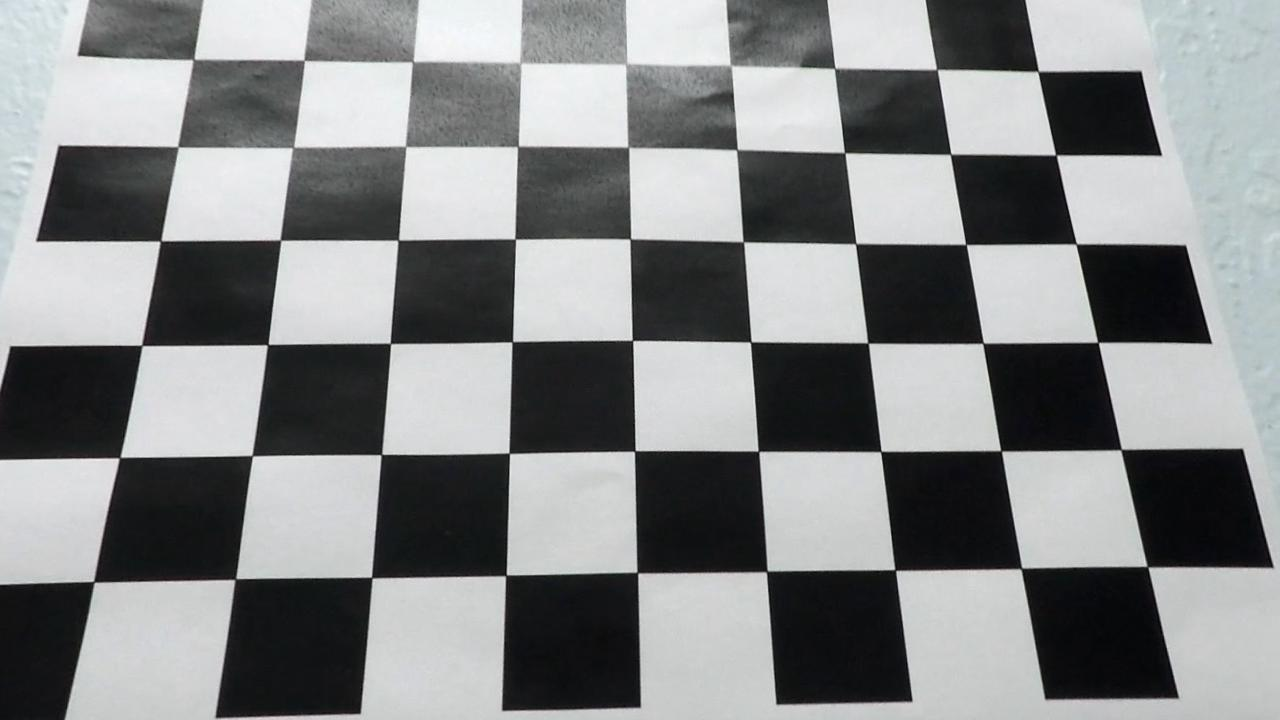
\includegraphics[width=0.5\textwidth]{output_images/calibration_result/calibration3/undistorted.jpg}\label{fig:distCorrf2}}
\caption{Result of the distortion correction on calibration image \cd+calibration3.jpg+.}
\label{fig:distCorr}
\end{figure}

\section{Perspective transform}
\label{sec:perspTr}
Perspective transform is performed from cell 14 to cell 16 (section \textit{Perspective transform}).

In cell 15 (executed cell 10) the matrices transformation are calculate using the image \cd+test_images/straight_lines1.jpg+. On this image, a trapezoid has been defined containing the straight lines of the image, whose points are defined in \cd+src+ array (for visualisation purposes, it is drawn over the original image). From an eye-bird point of view, the trapezoid corresponds to a rectangle whose width is equal to the bottom lane width in the image and height equal to the image height itself: these new coordinates are defined in \cd+dst+ array. The following source and destination points have been defined:

\begin{tabular}{ |M{4cm}||M{4cm}|  }
 \hline
 \multicolumn{2}{|c|}{Points used for perspective transform} \\
 \hline
Source points & Destination points \\
 \hline
(250, 680)   & (250, img1.shape[0])\\
(592, 450) &   (250, 0)\\
(690, 450( &(1060, 0)\\
(1060, 680)    &(1060, img1.shape[0])\\
 \hline
\end{tabular}

The transformation and inverse transformation matrices are calculated with:
\begin{lstlisting}
M = cv2.getPerspectiveTransform(src, dst)
Minv = cv2.getPerspectiveTransform(dst,src)
\end{lstlisting}
and are saved in \cd+output/persp_pickle.p+ pickle file as a dictionary to be retrieved later.

The image is transformed with the function:
\begin{lstlisting}
res_img = cv2.warpPerspective(img, M, (img.shape[1], img.shape[0]), flags=cv2.INTER_LINEAR)
\end{lstlisting}
Results of applying distortion correction and perspective transform on test images are contained in the folder \cd+output_images/perspective_transform+ (see the example \autoref{fig:perpTransf}).

\begin{figure}
\subfloat[Original image.]{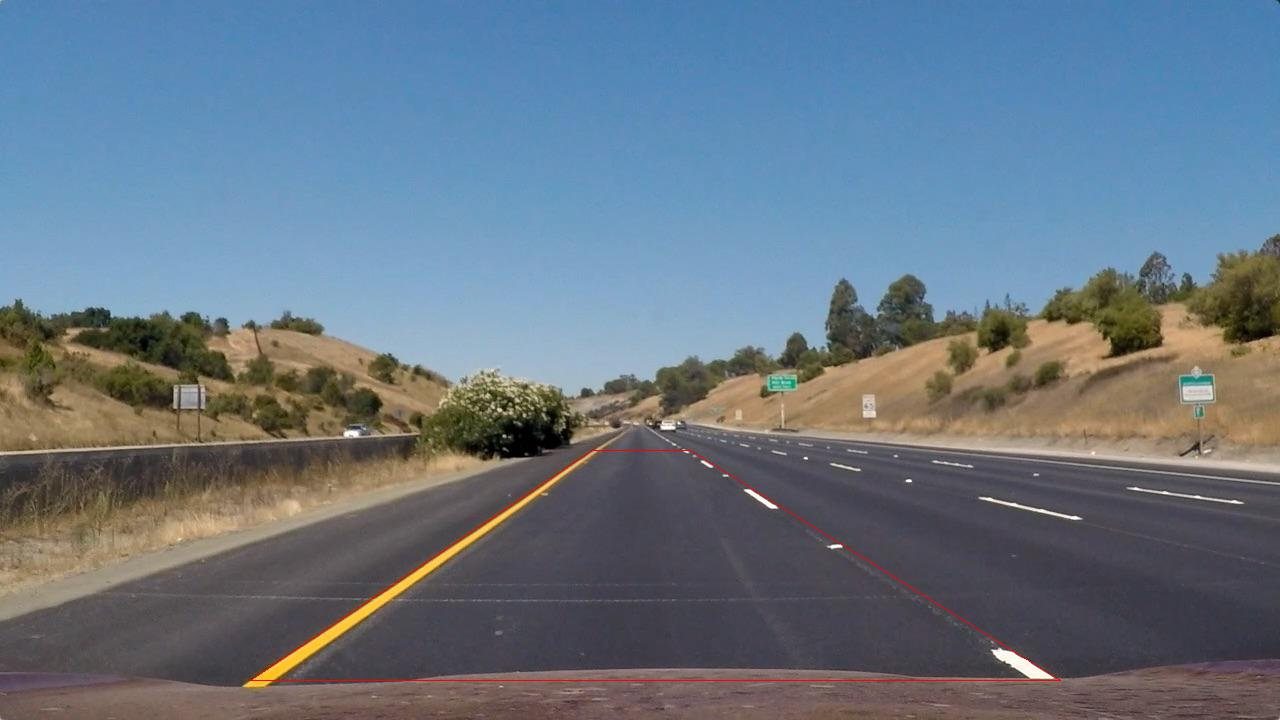
\includegraphics[width=0.5\textwidth]{output_images/perspective_transform/original.jpg}\label{fig:perpTransff1}}
\hfill
\subfloat[Eye-bird image.]{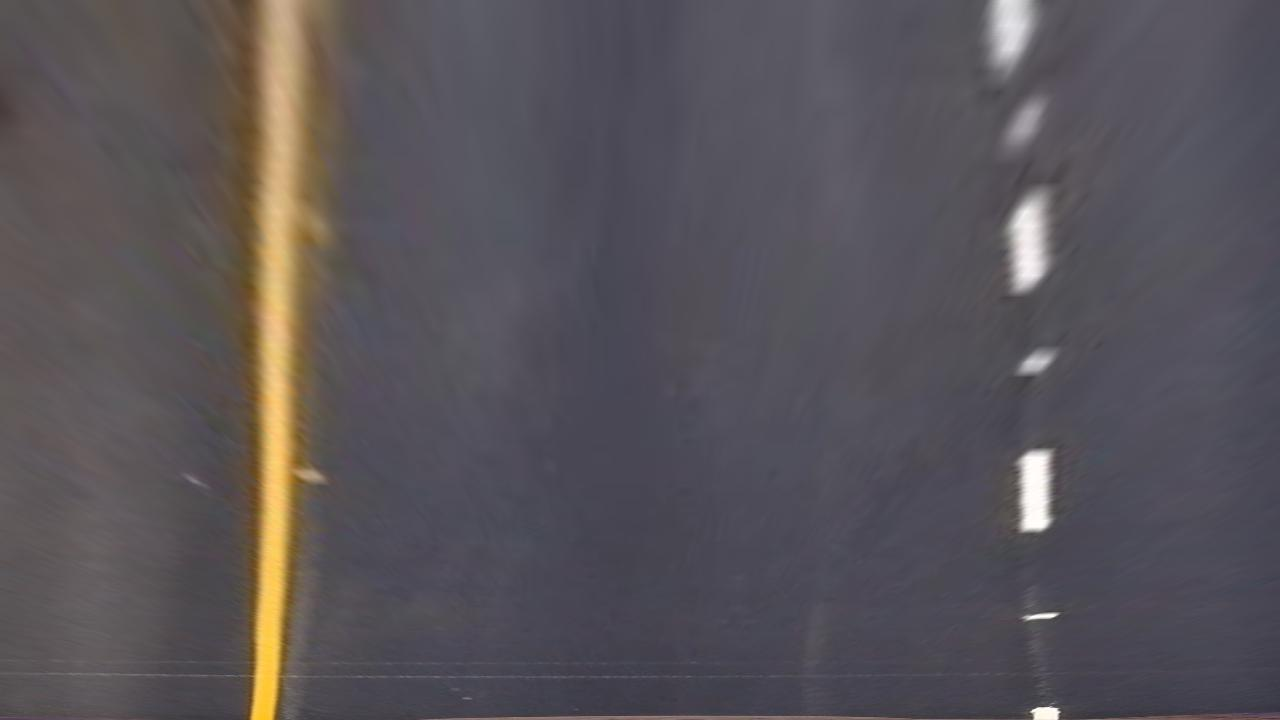
\includegraphics[width=0.5\textwidth]{output_images/perspective_transform/unwarped.jpg}\label{fig:perpTransff2}}
\caption{Result of the distortion correction and perspective transformation on test image \cd+straight_lines1.jpg+.}
\label{fig:perpTransf}
\end{figure}

\section{Pipeline description}
Now that all required matrices have been calculated, it is possible to define a pipeline consisting of the following steps:
\begin{enumerate}	
\item undistort the image;
\item perform magnitude thresholding to obtain a binary image;
\item perform colour thresholding to obtain a binary image;
\item combine the magnitude thresholding and colour thresholding binary images;
\item apply region of interest mask;
\item apply perspective transform; 
\item find pixel lanes;
\item fit two second order degree lines on pixel lanes;
\item calculate vehicle offset;
\item calculate line curvature;
\item draw the fitted lines and apply the inverse perspective transform.
\end{enumerate}

All the intermediate steps of the pipeline applied to the test images have been saved in \cd+output_images+, with each subfolder for each test image. This has been done in the loop contained in cell 28 (executed cell 17), section \textit{Analyse test images}. For demonstration purposes \cd+test_images/test1.jpg+ is considered (\autoref{fig:testimg}).
\begin{figure}
\centering
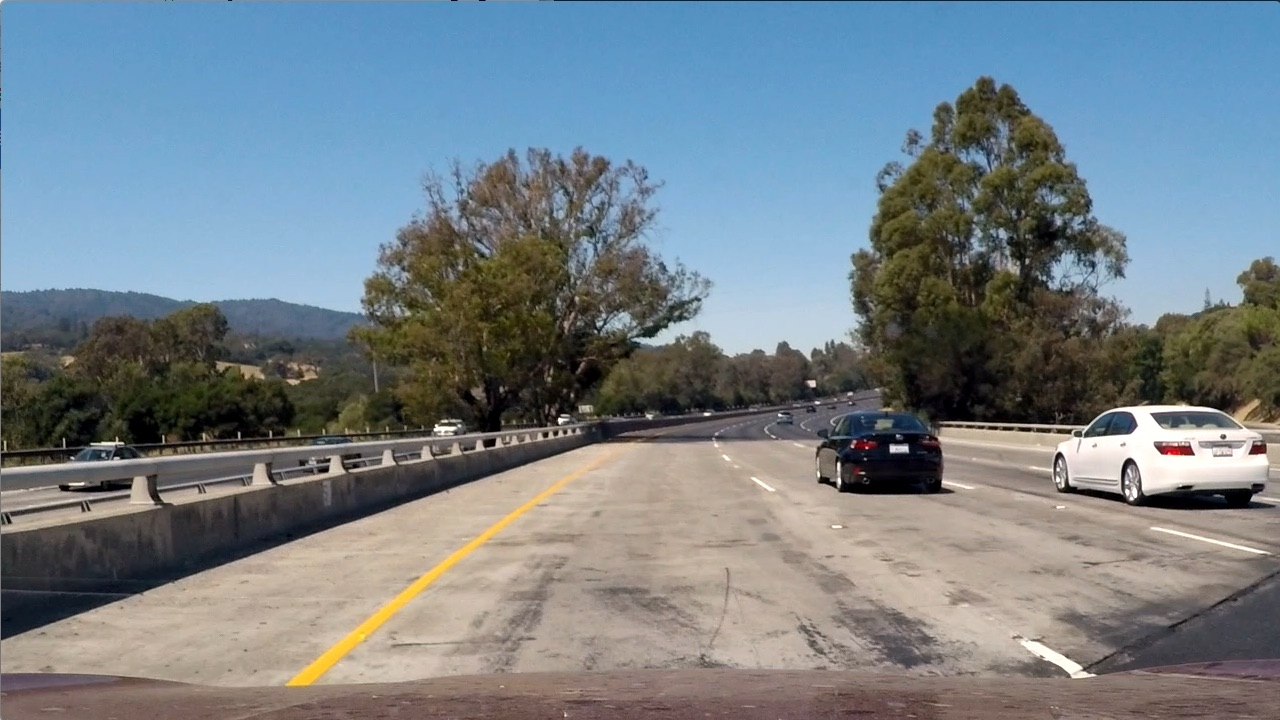
\includegraphics[scale=0.25]{test_images/test1}
\caption{Original image \cd+test1.jpg+ used to demonstrate the result of the pipeline.}
\label{fig:testimg}
\end{figure}

\subsection{Undistort the image}
As already told, this step is applied by calling \cd+cv2.undistort(image, mtx, dist, None, mtx);+. An example of this processing applied to the chosen image is shown in \autoref{fig:tstimg_dist}.
\begin{figure}
\centering
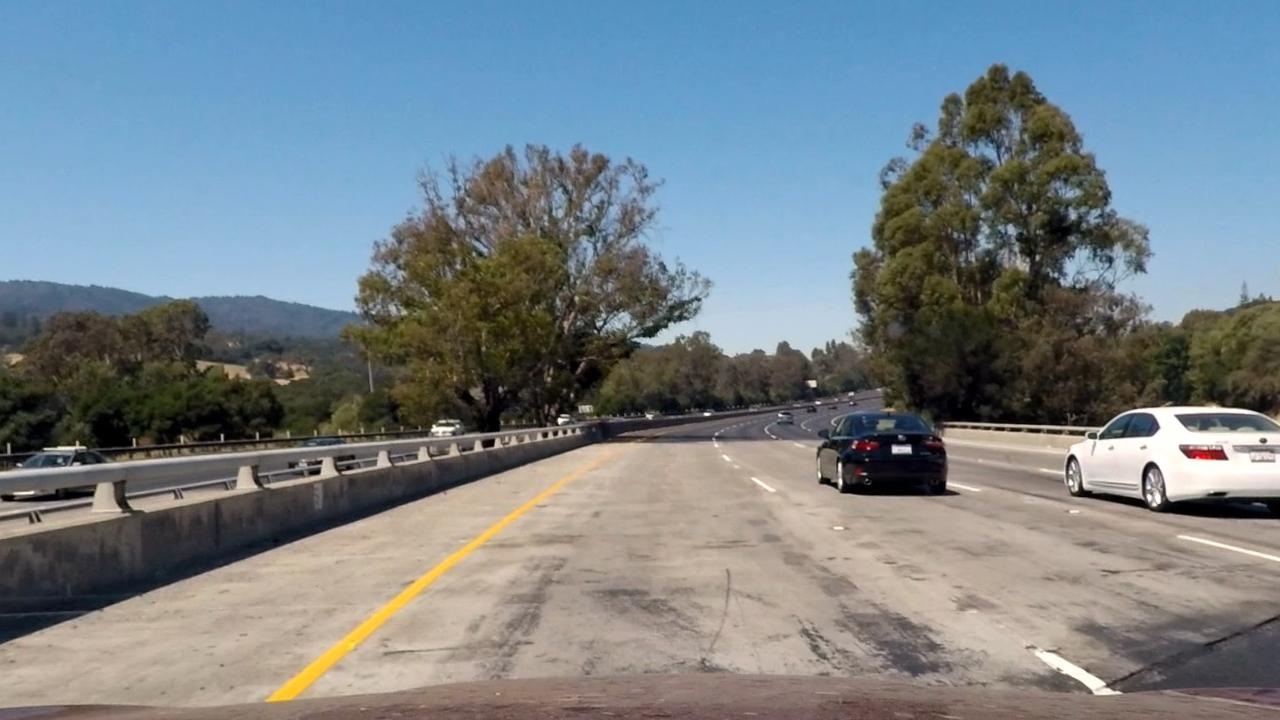
\includegraphics[scale=0.25]{output_images/test1/1_undistorted}
\caption{Undistorted image result.}
\label{fig:tstimg_dist}
\end{figure}

\subsection{Gradient thresholding}
The functions to perform gradient thresholds are defined in cell 18 (executed cell 12), section \textit{Magnitude functions}. The magnitude thresholding step has been defined with the function:
\begin{lstlisting}
def combine_magnitudes(img, ksize=3, k_size_dir=15, 
    sobel_thresh_x=(30, 100), sobel_thresh_y=(30, 100), 
    mag_thresh=(30, 100), dir_thresh=(0.85,1.15)):
  gradx = abs_sobel_thresh(img, orient='x', kernel_size=ksize, 
    thresh_min=sobel_thresh_x[0], thresh_max=sobel_thresh_x[1])
  grady = abs_sobel_thresh(img, orient='y', kernel_size=ksize, 
    thresh_min=sobel_thresh_y[0], thresh_max=sobel_thresh_y[1])
  mag_binary = mag_threshold(img, sobel_kernel=ksize, 
    mag_thresh=mag_thresh)
  dir_binary = dir_threshold(img, sobel_kernel=k_size_dir, 
    thresh=dir_thresh)
  combined_mag_thresholds = np.zeros_like(dir_binary)
  combined_mag_thresholds[((gradx == 1) & (grady == 1)) | 
    ((mag_binary == 1) & (dir_binary == 1))] = 1
  combined_mag_threshold_coloured = np.dstack(
    ( gradx, grady, dir_binary)) * 255
  return combined_mag_thresholds, combined_mag_threshold_coloured
\end{lstlisting}
\cd+abs_sobel_thresh+, \cd+mag_threshold+ and \cd+dir_threshold+ are the functions defined in the lectures so for seek of brevity they will not be reported here. The function simply calculates the derivatives along $x$ and $y$, the magnitude and the direction of  the gradient, taking for each component the absolute values and applying a minimum and maximum threshold to each independently. The threshold values are not too different from the ones used in the lectures. As suggested in the lecture, the individual resulting binary images are combined as:
\begin{lstlisting}
combined_mag_thresholds[((gradx == 1) & (grady == 1)) | 
  ((mag_binary == 1) & (dir_binary == 1))] = 1
\end{lstlisting}
The final result is shown in \autoref{fig:magThresh}. To see the contribution of its components and for debugging purposes, the function also returns an RGB image where the red channel is the derivative along $x$, the green channel the one along $y$ and the blue channel is the direction threshold analysis (\autoref{fig:magThreshCol}).
\begin{figure}
\centering
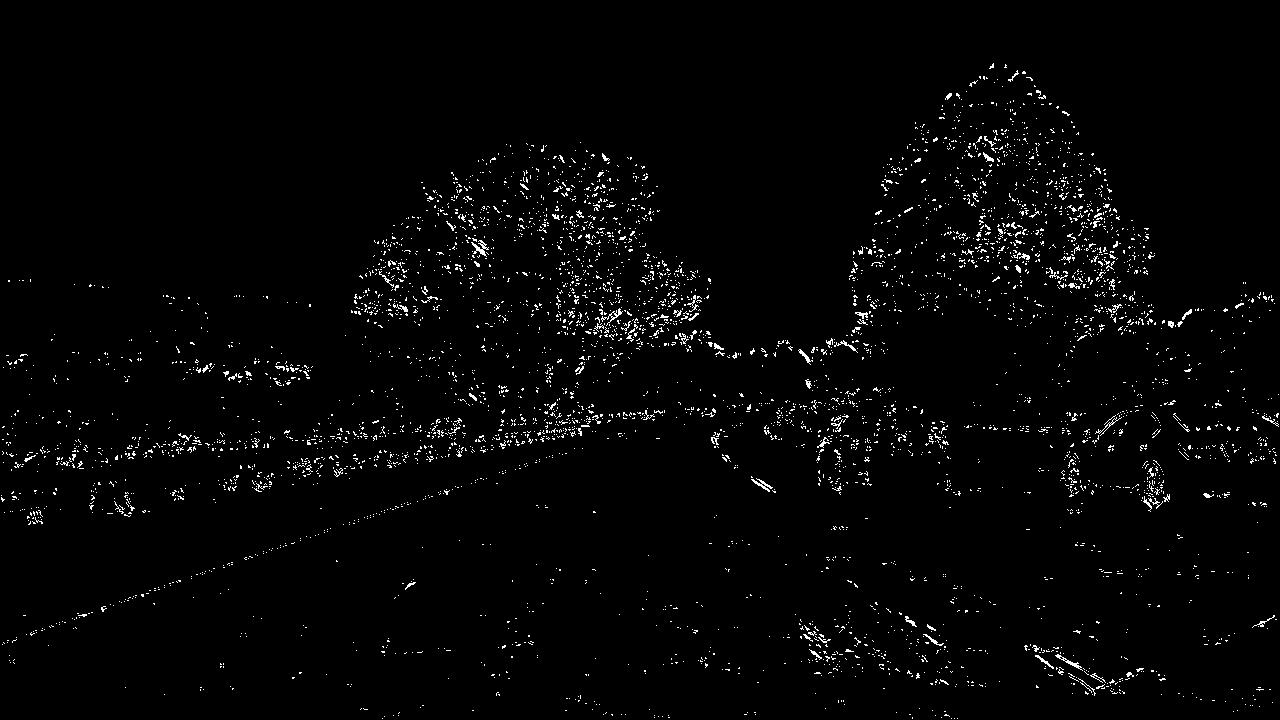
\includegraphics[scale=0.25]{output_images/test1/3_mag_threshold_bin}
\caption{Example of binary image resulting from the magnitude threshold analysis.}
\label{fig:magThresh}
\end{figure}
\begin{figure}
\centering
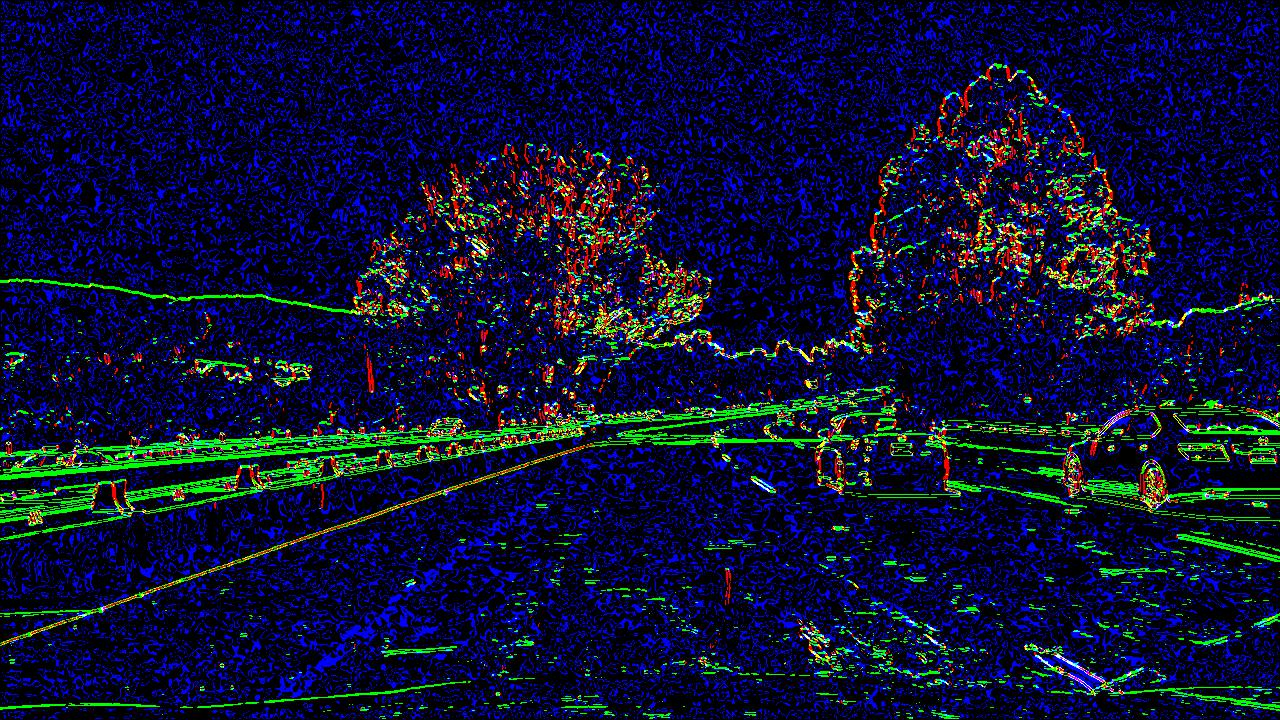
\includegraphics[scale=0.25]{output_images/test1/2_mag_threshold_coloured}
\caption{Example of RGB image returned by the function \cd+combine_magnitudes+ where the red channel is the derivative along $x$, the green channel the one along $y$ and the blue channel is the direction threshold analysis.}
\label{fig:magThreshCol}
\end{figure}


\subsection{Colour threshold}
Instead of applying colour thresholding on the RGB space, it is easier to apply them in the HLS or HSV space. In cell 23 (executed cell 14), section \textit{ Find colour threshold values}, the HLS and HSV channels are shown in two images in the RGB space. From \autoref{fig:HLSvsHSV}, it seems that white lane detection seems more straightforward in the HLS space, so we will perform the analysis in this space.

\begin{figure}
\centering
\subfloat[HLS channels displayed in the RGB space]{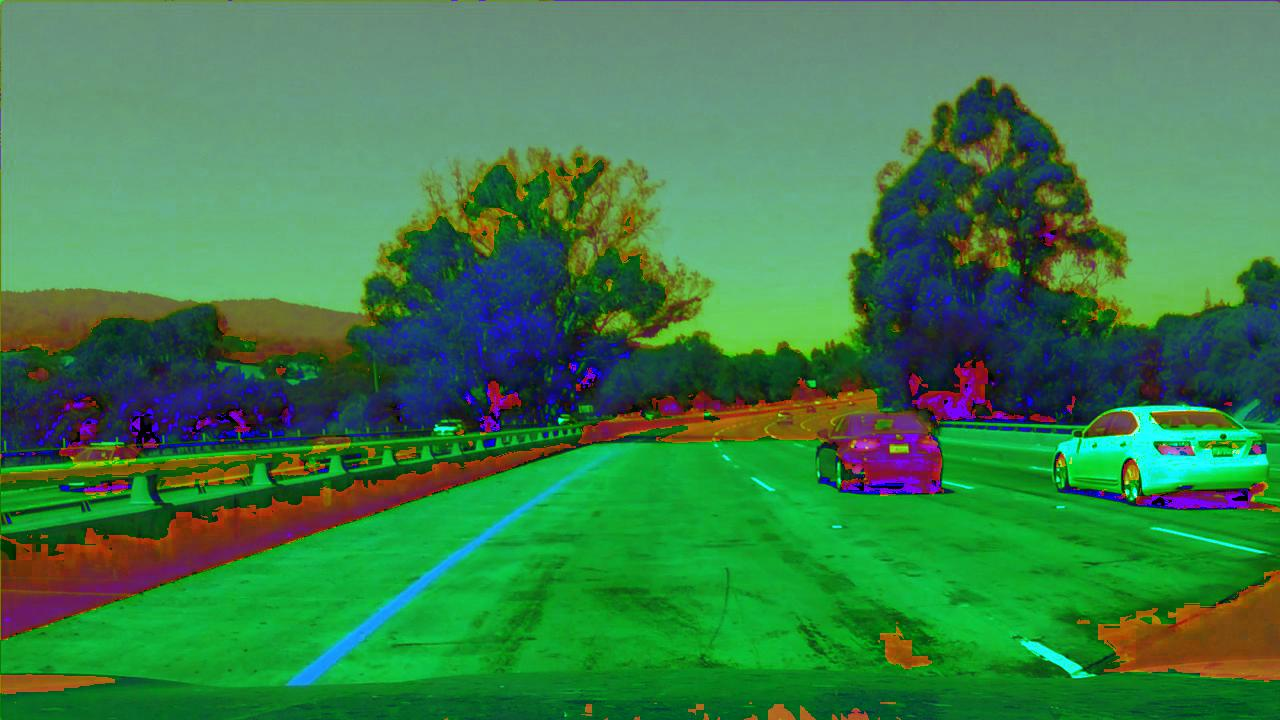
\includegraphics[width=0.5\textwidth]{output_images/HLSvsHSV/hls}\label{hls}}
\subfloat[HSV channels displayed in the RGB space]{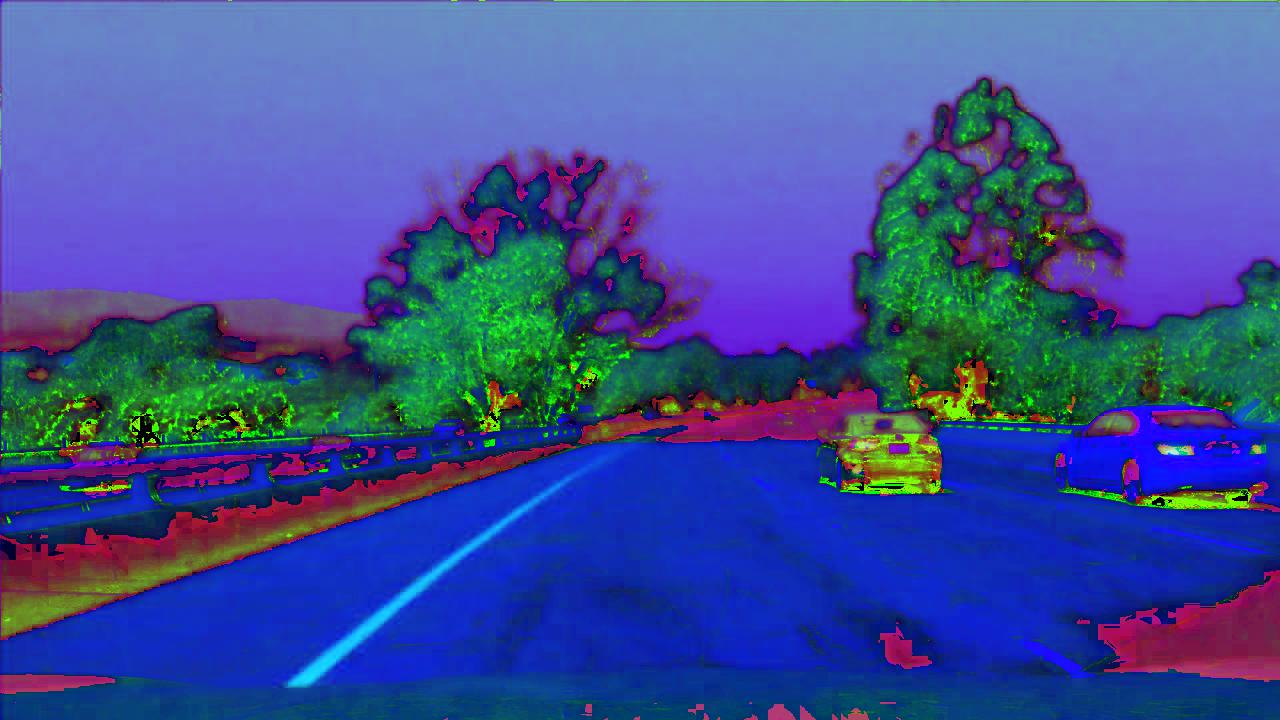
\includegraphics[width=0.5\textwidth]{output_images/HLSvsHSV/hsv}\label{hsv}}
\caption{Comparison between HLS and HSV colour space.}
\label{fig:HLSvsHSV}
\end{figure}

To perform the colour threshold the function \cd+colour_threshold+ has been defined in cell 18 (executed cell 12), section \textit{Magnitude functions}:
\begin{lstlisting}
def colour_threshold(img, s_thresh=(150, 255),
   l_thresh=(150, 255), h_thresh=(120,250), v_thresh=(180,250)):
  hls = cv2.cvtColor(img, cv2.COLOR_RGB2HLS)
  h_channel = hls[:,:,0]
  l_channel = hls[:,:,1]
  s_channel = hls[:,:,2]
  # Convert to HSV
  hsv = cv2.cvtColor(img, cv2.COLOR_RGB2HSV)
  v_channel = hsv[:,:,2]

  s_binary = np.zeros_like(s_channel)
  s_binary[(s_channel >= s_thresh[0]) & (s_channel <= s_thresh[1])] = 1
    
  l_binary = np.zeros_like(l_channel)
  l_binary[(l_channel >= l_thresh[0]) & (l_channel <= l_thresh[1])] = 1

  h_binary = np.zeros_like(h_channel)
  h_binary[(h_channel >= h_thresh[0]) & (h_channel <= h_thresh[1])] = 1
    
  v_binary = np.zeros_like(v_channel)
  v_binary[(v_channel >= v_thresh[0]) & (v_channel <= v_thresh[1])] = 1
  # Stack each channel to view their individual contributions in green and blue respectively
  # This returns a stack of the two binary images, whose components you can see as different colors
  colour_binary_stacked_hls = np.dstack(( h_binary, l_binary, s_binary)) * 255
  colour_binary_stacked_hsv = np.dstack(( h_binary, s_binary, v_binary)) * 255

  # Combine the two binary thresholds
  combined_colour_binary = np.zeros_like(s_binary)
  combined_colour_binary[((h_binary==1)&(s_binary==1)&(l_binary==1))] = 1
  return combined_colour_binary, colour_binary_stacked_hls, colour_binary_stacked_hsv
\end{lstlisting}
The function converts the RGB image into the HLS and HSV representations. Each channel is thresholded to obtain a binary image from each of them. Then a single binary image is returned by performing pixelwise AND on the H,L and S channels. For visualisation and debugging purposes, the function returns also the previously seen HLS and HSV representations displayed in the RGB space, understand the contribution of each channel separately.

The function is called three times with different thresholds from the pipeline: one to get the yellow lane, one to get the white lane and a third time to get some other parts of the white lane that are difficult to find, the parts that are further ahead. Then the three resulting images are pixelwise ORed:
\begin{lstlisting}
h_thresh_yellow=(0, 30)
l_thresh_yellow=(80, 190)
s_thresh_yellow=(150, 255)

h_thresh_white=(0, 170)
l_thresh_white=(100, 255)
s_thresh_white=(100, 255)

h_thresh_white2=(130, 170)
l_thresh_white2=(160, 240)
s_thresh_white2=(0, 150)
yellow_lane, _, _ = colour_threshold(undistort_img, 
  h_thresh=h_thresh_yellow, l_thresh=l_thresh_yellow,
  s_thresh=s_thresh_yellow)
white_lane, _, _ = colour_threshold(undistort_img, 
  h_thresh=h_thresh_white, l_thresh=l_thresh_white,
  s_thresh=s_thresh_white)
white_lane2, _, _ = colour_threshold(undistort_img, 
  h_thresh=h_thresh_white2, l_thresh=l_thresh_white2,
  s_thresh=s_thresh_white2)
combined_colour_thr_binary = white_lane | white_lane2 |
  yellow_lane
\end{lstlisting}
The result is shown in \autoref{fig:colThresh}.
\begin{figure}
\centering
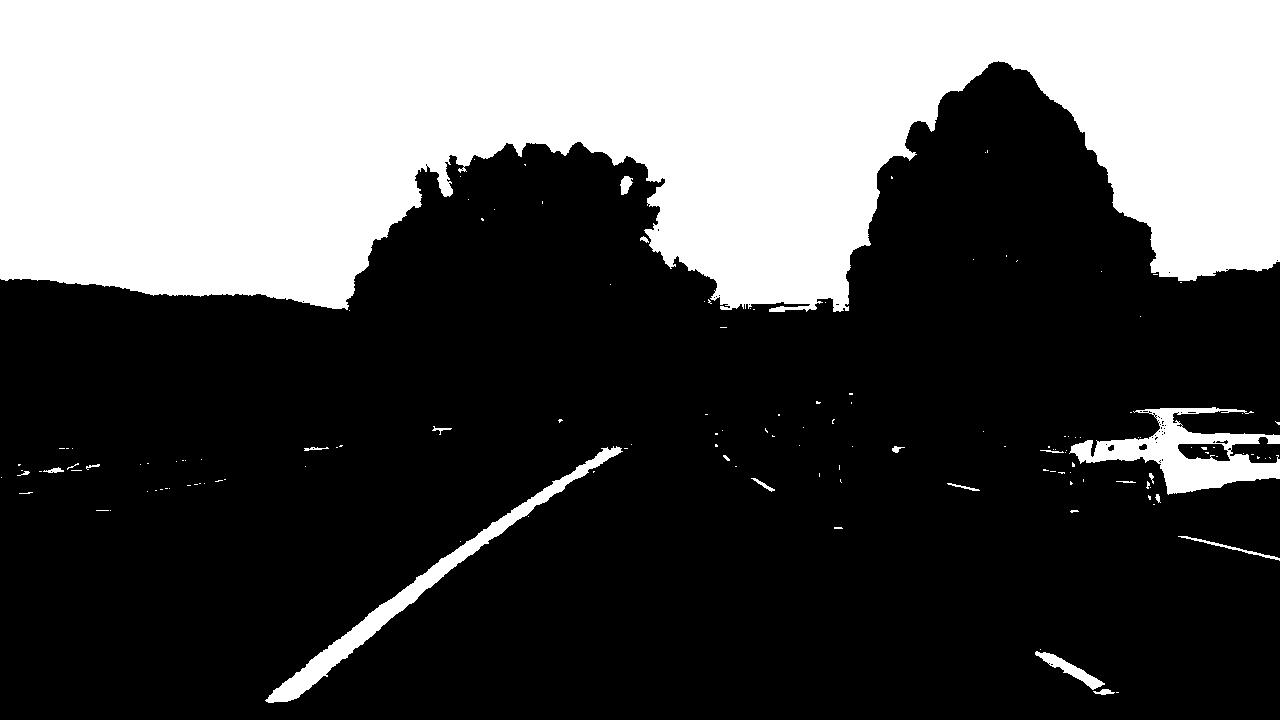
\includegraphics[scale=0.25]{output_images/test1/5_col_threshold_bin}
\caption{Binary image resulting from colour thrsholding}
\label{fig:colThresh}
\end{figure}

\subsubsection{Finding the colour thresholds}
To find the colour thresholds, cell 26 (executed cell 16) plots the HLS and HSV representations in the colour space using \cd+\%matplotlib tk+ backend, so that it is possible to hover with the mouse over the pixels to check their value and get an idea of the thresholds.

\subsection{Combine the two thresholds}
The binary image resulting from gradient thresholding and the one resulting from colour thresholding are pixelwise ORed to get a single image.
\begin{lstlisting}
combined_binary = np.zeros_like(combined_mag_thresholds)
combined_binary[(combined_colour_thr_binary == 1) | 
  (combined_mag_thresholds == 1)] = 1
\end{lstlisting}
Result is shown in \autoref{fig:combined}.
\begin{figure}
\centering
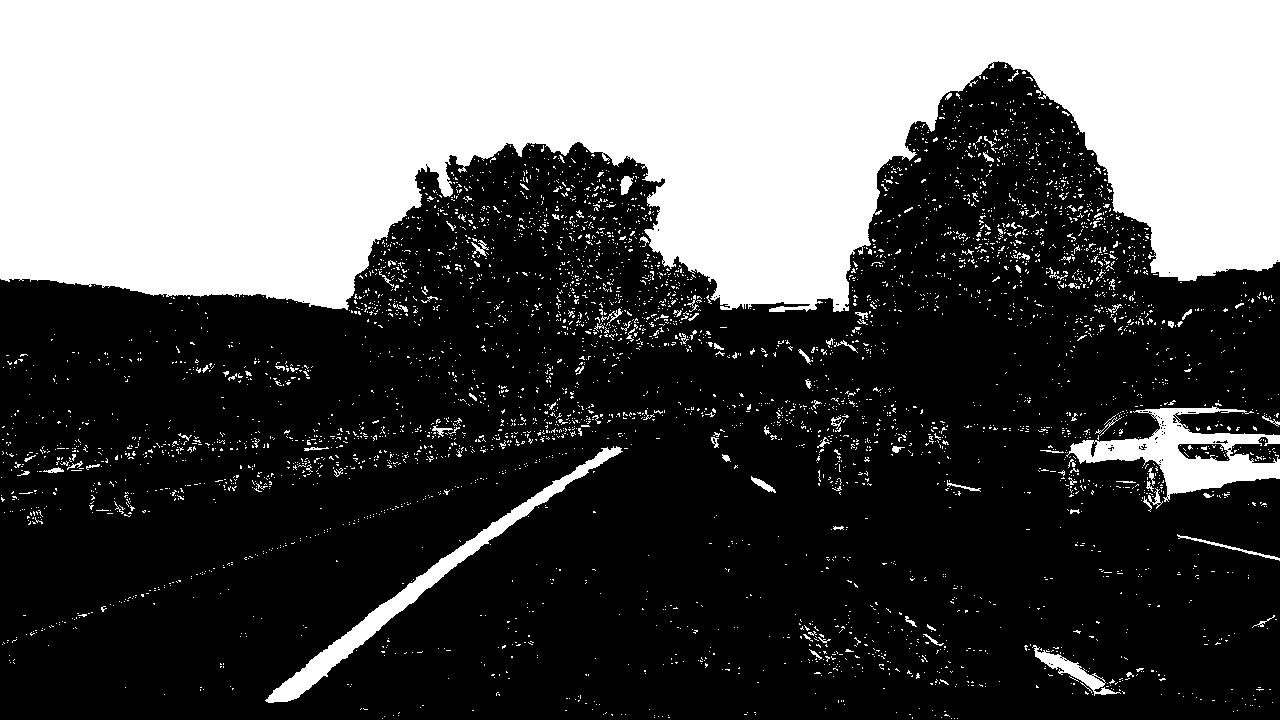
\includegraphics[scale=0.25]{output_images/test1/6_combined_mag_colour_threshold}
\caption{Binary image resulting from the combination of gradient thresholding step and colour thresholding step.}
\label{fig:combined}
\end{figure}

\subsection{Region of interest selection}
The region of interest has been explained in the previous project. The vertices used in this case are the following:
\begin{lstlisting}
vertices = np.array([[[int(xsz*0.1), ysz], [int(xsz*0.95), ysz], 
    [int(0.56*xsz), int(0.61*ysz)],
    [int(0.48*xsz), int(0.61*ysz)]]])
\end{lstlisting}	
The result is shown in \autoref{fig:regOfInterest}.
\begin{figure}
\centering
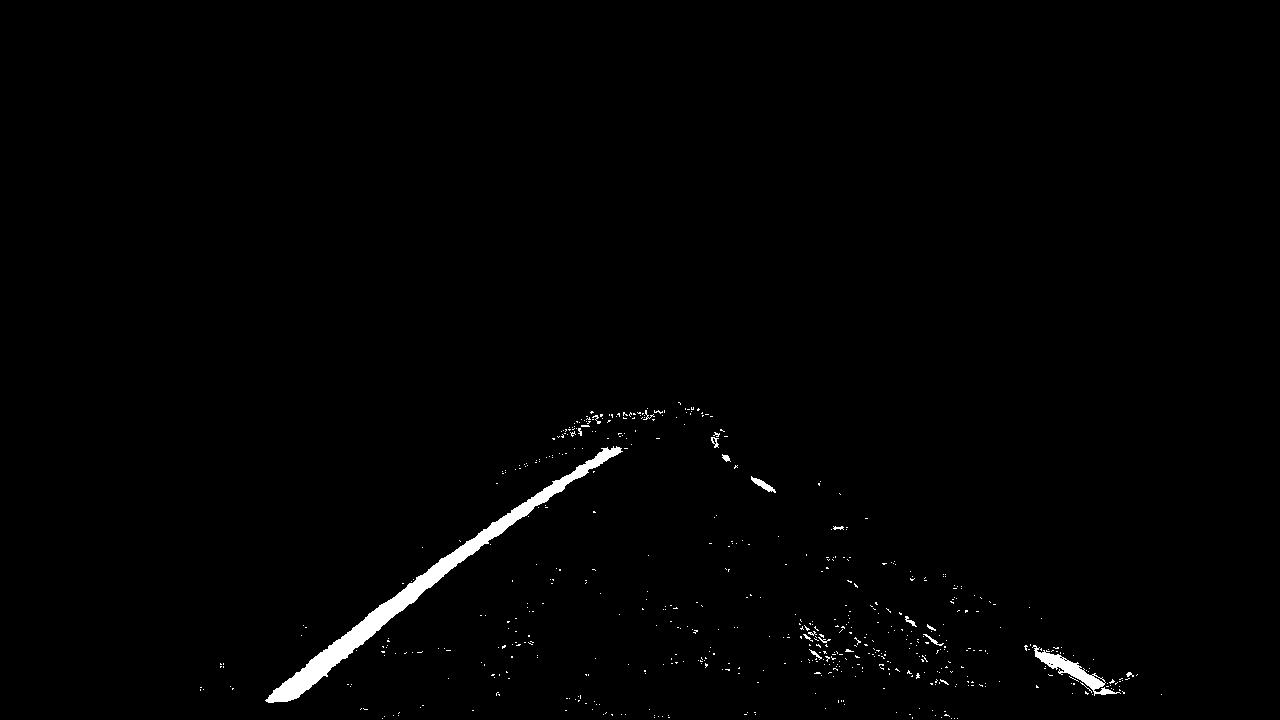
\includegraphics[scale=0.25]{output_images/test1/7_region_of_interest}
\caption{Binary image the region of interest mask.}
\label{fig:regOfInterest}
\end{figure}

\subsection{Apply perspective transform}
The perspective transform has already been explained in \autoref{sec:perspTr}. The result is shown in \autoref{fig:perspTrPipe}
\begin{figure}
\centering
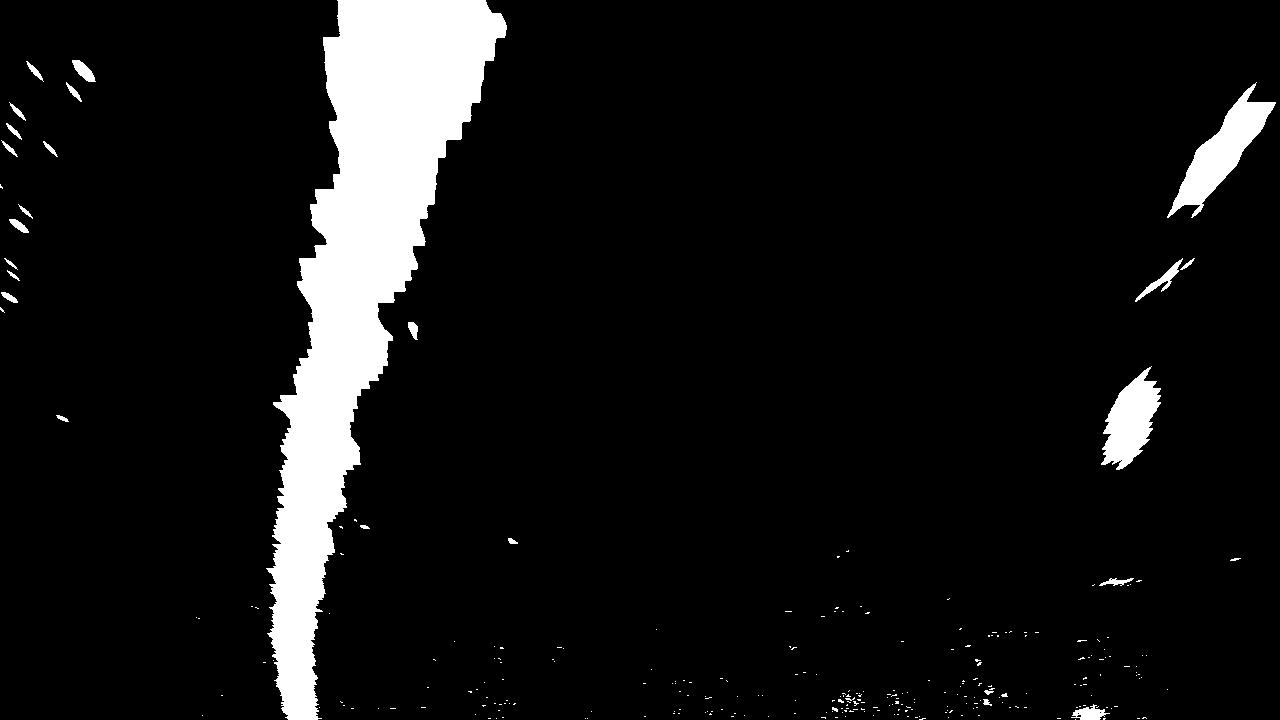
\includegraphics[scale=0.25]{output_images/test1/8_persp_transf}
\caption{Image resulting from the perspective transformation.}
\label{fig:perspTrPipe}
\end{figure}

\subsection{Find the lanes pixels}
The lanes pixels are found by the function \cd+find_lane_pixels+ defined in the cell 20 (execution cell 13), section \textit{Functions for lane detection}. The function takes as input the warped binary image, but it must be rescaled so the non-zero values are $255$: it is sufficient to multiply the binary image by 255 for this. The function has been explained in the lecture. It takes a histogram of the bottom half of the image with the call \cd+histogram = np.sum(binary_warped[binary_warped.shape[0]//2:,:], axis=0)+. The histogram is expected to have two peaks, one on left side and one on the right that are found with the piece of code:
\begin{lstlisting}
midpoint = np.int16(histogram.shape[0]//2)
leftx_base = np.argmax(histogram[:midpoint])
rightx_base = np.argmax(histogram[midpoint:]) + midpoint
\end{lstlisting} 
To find the lane pixels two series of windows one above the other have to be defined, one for each lane: the active pixels that will lie within these windows will constitute the lane pixels. We start by defining one window for each lane at the bottom of the image having the same $x$ coordinate of the peak (its width and height are hyperparameters). The non-zero pixels that lie within this window are the first lane pixels. The next window is positioned above the other but it might be recentred: if the number of pixels within the previous window is above the threshold \cd+min_pix+, their mean is used to recentre the next window; if not the old position is used. The lines of code in the function that do this are the following:
\begin{lstlisting}
nwindows = 9
# Set the width of the windows +/- margin
margin = 100
# Set minimum number of pixels found to recenter window
minpix = 50

leftx_current = leftx_base # max of the left part histogram
rightx_current = rightx_base # max of the right histogram

# Create empty lists to receive left and right lane pixel indices
left_lane_inds = []
right_lane_inds = []

# Step through the windows one by one
for window in range(nwindows):
  # Identify window boundaries in x and y (and right and left)
  win_y_low  = binary_warped.shape[0] - (window+1)*window_height
  win_y_high = binary_warped.shape[0] -  window   *window_height
  ### TO-DO: Find the four below boundaries of the window ###
  win_xleft_low  = leftx_current - margin 
  win_xleft_high = leftx_current + margin  
  win_xright_low = rightx_current - margin
  win_xright_high = rightx_current + margin 
  
  # Identify the nonzero pixels in x and y within the window #

  good_left_inds = ((nonzeroy >= win_y_low) & (nonzeroy < win_y_high) & 
      (nonzerox >= win_xleft_low) &  (nonzerox < win_xleft_high)).nonzero()[0]
  good_right_inds = ((nonzeroy >= win_y_low) & (nonzeroy < win_y_high) & 
      (nonzerox >= win_xright_low) &  (nonzerox < win_xright_high)).nonzero()[0]
  if len(good_left_inds) > minpix:
    leftx_current = np.int16(np.mean(nonzerox[good_left_inds]))
  if len(good_right_inds) > minpix:        
     rightx_current = np.int16(np.mean(nonzerox[good_right_inds]))
\end{lstlisting}


The total number of windows is given by the height of the image divided by the height of the window. The visualisation of this step is shown in \autoref{fig:lanePix}
\begin{figure}
\centering
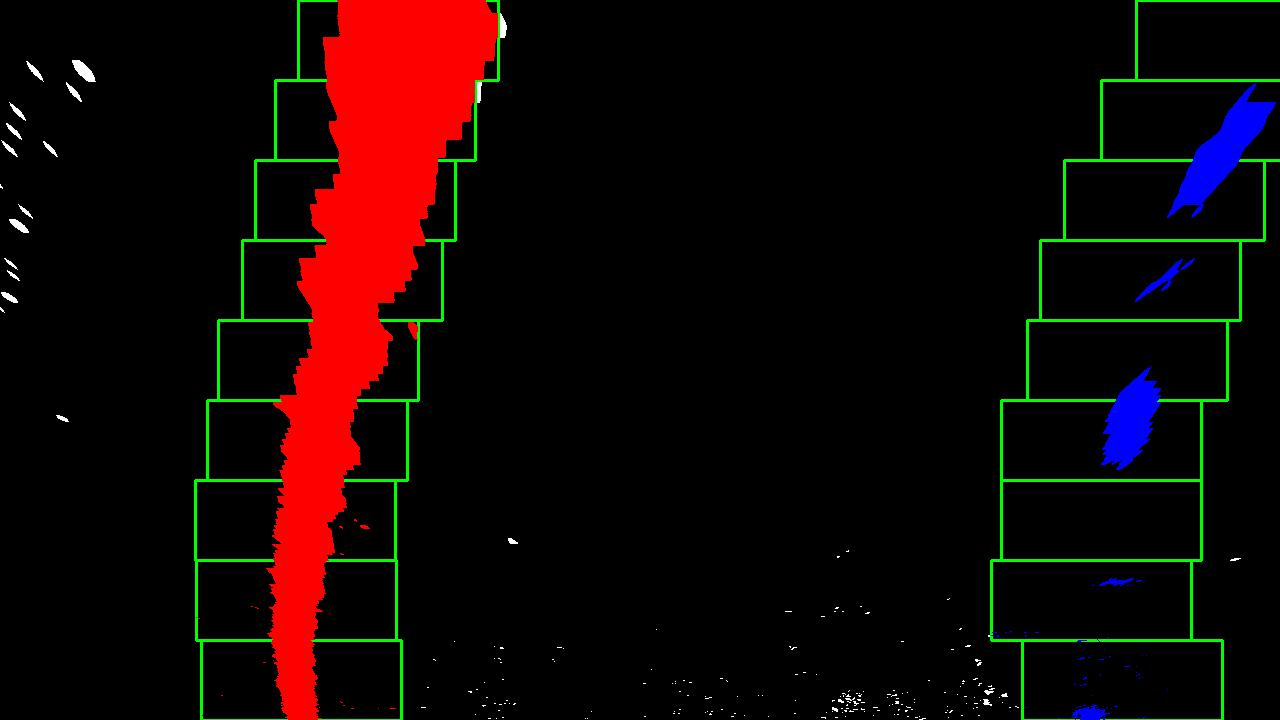
\includegraphics[scale=0.25]{output_images/test1/9_windowed}
\caption{Image showing the windows to classify the left lane pixels in red, the right lane pixels in blue and the non-lane pixels in white.}
\label{fig:lanePix}
\end{figure}

\subsection{Fit the second degrees line}
The function that fits the left and right lines is \cd+fit_polynomial+ defined in the cell 20 (execution cell 13), section \textit{Functions for lane detection}. This function calls \cd+find_lane_pixels+: whereas \cd+find_lane_pixels+ is explicitly called when analysing the test images to show the result of the process, in the video pipeline it will be called only from \cd+fit_polynomial+. After finding the lane pixels by calling \cd+find_lane_pixels(..)+, the function fits the second order polynomials by calling \cd+np.polyfit(y, x, deg=2)+ ($y$ is the axis along the height of the image, $x$ the one along its width) which returns the polynomial coefficients. Then the line points are calculated and draw on the image in cyan with the code:
\begin{lstlisting}
ploty = np.linspace(0, binary_warped.shape[0]-1, binary_warped.shape[0] )
try:
  left_fitx = left_fit[0]*ploty**2 + left_fit[1]*ploty + left_fit[2]
  right_fitx = right_fit[0]*ploty**2 + right_fit[1]*ploty + right_fit[2]
except:
...
cv2.polylines(out_img, [pts_left], False, color=(0,255,255),  thickness=5)
cv2.polylines(out_img, [pts_right], False, color=(0,255,255), thickness=5)
\end{lstlisting}
The result is shown in \autoref{fig:fitPoly}.
\begin{figure}
\centering
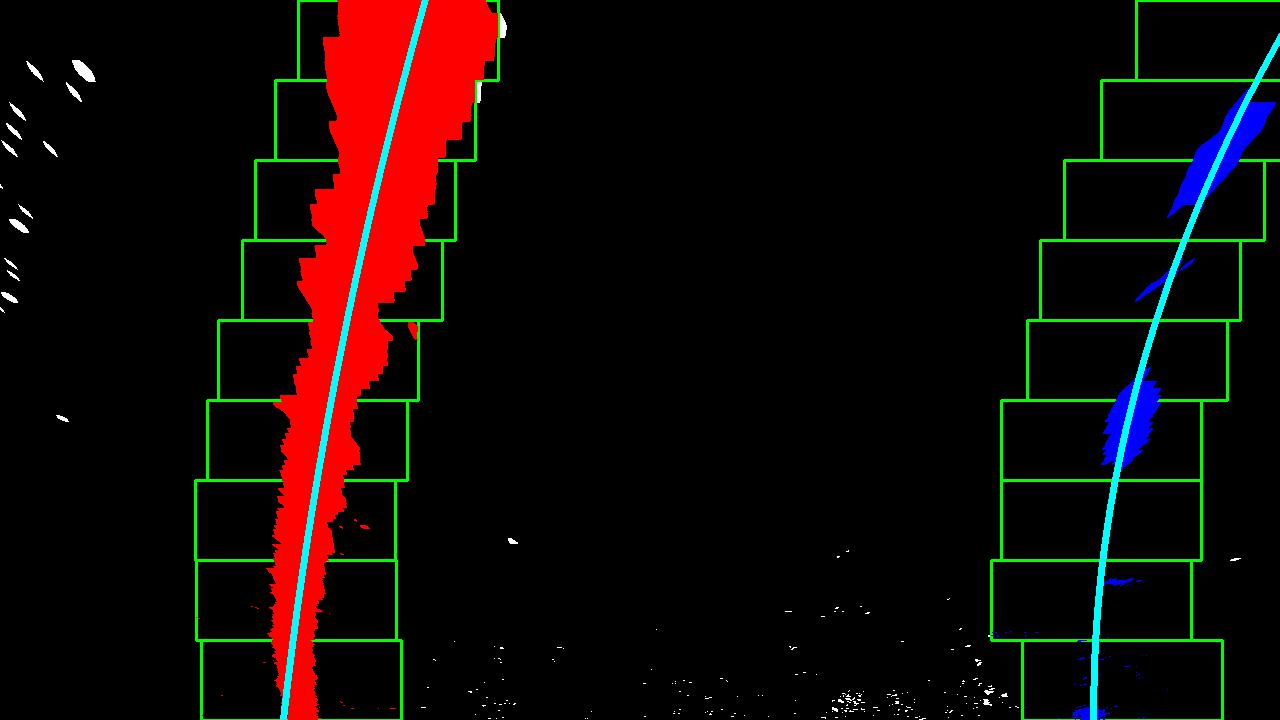
\includegraphics[scale=0.25]{output_images/test1/10_fit_polynomial}
\caption{Image showing result of fitting two second degrees polynomial on each lane pixels.}
\label{fig:fitPoly}
\end{figure}

\subsection{Vehicle offset}
The vehicle offset is calculated with the function \cd+vehicle_offset+ defined in the cell 20 (execution cell 13), section \textit{Functions for lane detection}
\begin{lstlisting}
def vehicle_offset(left_fit, right_fit, shape):
  global xm_per_pix
  lane_center = ((left_fit[0] + right_fit[0])*shape[0]**2 + 
    (left_fit[1] + right_fit[1])*shape[0] +
    left_fit[2] + right_fit[2])//2
  car_center = shape[1]/2  # we assume the camera is centered in the car
  center_offset = (lane_center - car_center) * xm_per_pix
  return center_offset
\end{lstlisting}
The function calculates the centre of the lane and the car centre, subtracts them and converts the result from pixels to metres. The car centre is half the width of the image (since the camera is supposed to be mounted exactly on the midpoint of the car). To calculate the lane centre, the function sums the values of the lines at the bottom of the image and divides it by two. In my case the lines have the abscissa starting at the top of the image, so their value is calculated with the input \cd+shape[0]+, where \cd+shape+ is the image shape.

The result is printed on the resulting image itself together with radius of curvature of the two lines and other information (see \autoref{fig:final}).

\subsection{Line curvature}
The curvature of each line is calculated using the efficient method described in the lecture and implemented in the function \cd+measure_curvature_efficient+, defined in the cell 20 (execution cell 13), section \textit{Functions for lane detection}, that converts the line coefficients before applying the curvature equation. The coefficients are converted to get a value in metres by the following code:

\begin{lstlisting}
left_fit_cp = left_fit.copy()
right_fit_cp = right_fit.copy()
left_fit_cp[0] = left_fit[0]* xm_per_pix/(ym_per_pix**2)
left_fit_cp[1] = left_fit[1]* xm_per_pix/(ym_per_pix)
right_fit_cp[0] = right_fit[0]* xm_per_pix/(ym_per_pix**2)
right_fit_cp[1] = right_fit[1]* xm_per_pix/(ym_per_pix)
\end{lstlisting}
Then the equation described in the lecture is applied.
The result is printed on the resulting image itself together with vehicle offset and other information (see \autoref{fig:final}).

\begin{figure}
\centering
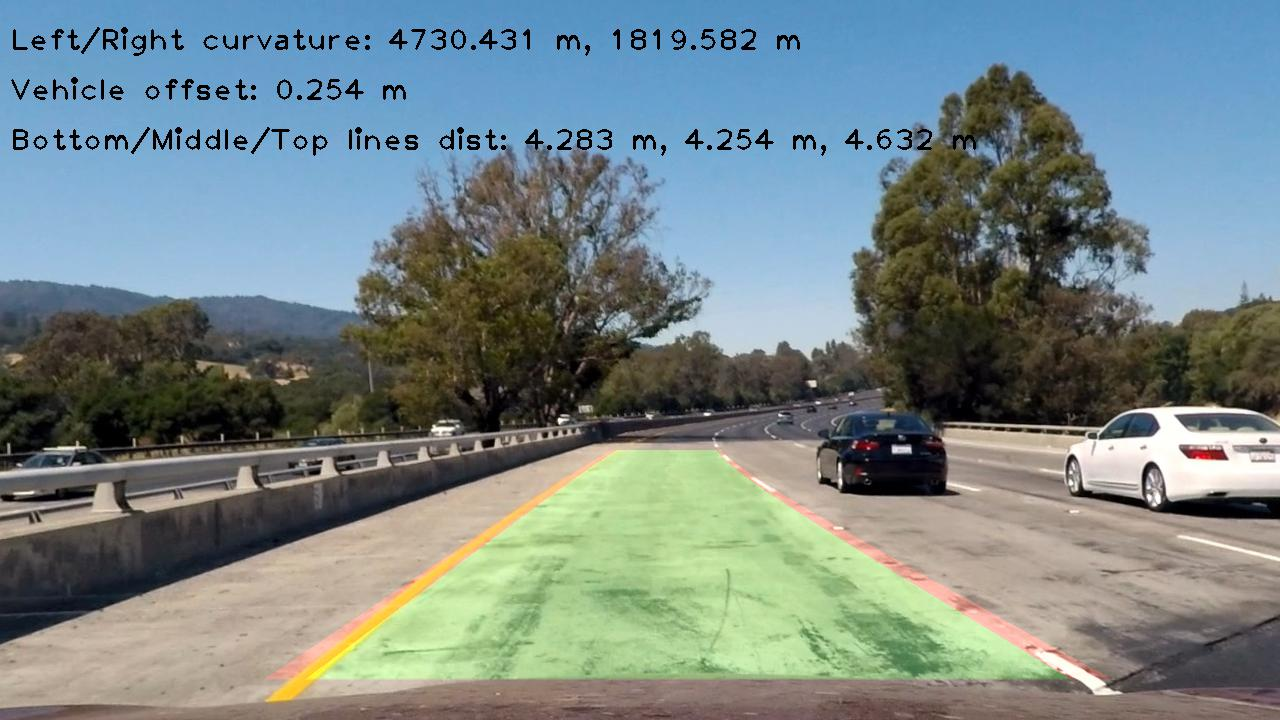
\includegraphics[scale=0.25]{output_images/test1/11_unwarped_lanes}
\caption{Final result of the pipeline.}
\label{fig:final}
\end{figure}

\subsection{Draw the fitted lines and apply the inverse perspective transform}
For this step, first an empty image is created where the two lines are dawn, then the inverse perspective transform is applied to this image and the result is merged with the undistorted image. The code which does this starts from line $127$ of the cell $28$ responsible for analysing the test images (section \textit{Analyse test images}):
\begin{lstlisting}
rev_img = np.zeros_like(undistort_img)
cv2.polylines(rev_img, [points_left], False, color=(255,0,0), thickness=40)
cv2.polylines(rev_img, [points_right], False, color=(255,0,0), thickness=40)
unwarped_lanes = cv2.warpPerspective(rev_img, Minv, (rev_img.shape[1], rev_img.shape[0]), 
  flags=cv2.INTER_LINEAR)
result = weighted_img(initial_img=undistort_img, img=unwarped_lanes) 
\end{lstlisting}
\cd+weighted_img+ has also been used in the first project. The final result is shown in \autoref{fig:final}.

\section{Video pipeline}
The pipeline steps have been grouped into a function to be called when analysing the video. Two versions have been implemented: a simple one consisting of the previously described steps and an advanced version which implements sanity check and that searches line pixels around the line fitted on the previous video frame so as to save computation by avoiding performing the hystogram analysis each time.

\subsection{Simple version of the pipeline video}
The pipeline video steps are implemented in the function \cd+pipeline(image)+ defined in cell 29 (executed cell 18). The steps are identical to the previous ones, except that \cd+find_lane_pixels+ is not explicitly called, since the function \cd+fit_polynomial+ is responsible for this call.

For debugging and visualisation purposes, some intermediate steps of the pipeline are shown on the top right of the video, so that one can get a larger picture of what is going on behind the curtains. The lines of code responsible for this are the following:
\begin{lstlisting}
scale_percent = 20 # percent of original size
width = int(combined_binary.shape[1] * scale_percent / 100)
height = int(combined_binary.shape[0] * scale_percent / 100)
dim = (width, height)
# plot resized images from the analysis on top right for debugging purposes
resized = cv2.resize(res_img, dim, interpolation = cv2.INTER_AREA)
resized2 = cv2.resize(warped_binary_white, dim, interpolation = cv2.INTER_AREA)
resized3 = cv2.resize(combined_binary_white, dim, interpolation = cv2.INTER_AREA)
resized4 = cv2.resize(region_of_intrst_white, dim, interpolation = cv2.INTER_AREA)

result[:height, result.shape[1]-2*width:result.shape[1]-width] = weighted_img(initial_img=resized2, 
    img=result[:height, result.shape[1]-2*width:result.shape[1]-width], alpha=1, beta=0.5)
result[:height, result.shape[1]-width:result.shape[1]] = weighted_img(initial_img=resized, 
    img=result[:height, result.shape[1]-width:result.shape[1]], alpha=1, beta=0.5)
result[height:2*height, result.shape[1]-2*width:result.shape[1]-width] = weighted_img(initial_img=resized3, 
    img=result[height:2*height, result.shape[1]-2*width:result.shape[1]-width], alpha=1, beta=0.5)
result[height:2*height, -width:] = weighted_img(initial_img=resized4, 
    img=result[height:2*height, -width:], alpha=1, beta=0.5)
\end{lstlisting}
Basically, the images resulting from the intermediate steps of the pipeline to be shown are downsampled and blended with the pixels of the top right region of the final image of the pipeline.

\subsubsection{Video output}
The output video of the project is in \cd+output/project_video.mp4+ \href{https://github.com/FrancescoBoi/AdvancedLaneDetection/blob/master/output/project_video.mp4}{and it can be downloaded from this link}.

\subsection{Advanced Video pipeline}
The new pipeline steps are implemented in the function \cd+pipeline_advanced(image)+ defined in cell 30 (executed cell 19). Steps 1 through 6 are the same of the previous pipeline.

\subsubsection{Line class}
As suggested in the lecture, a class \cd+Line+ has been defined in cell 30 (executed cell 19). The goal of this class is to average the last fitted lines so as to get a better result by smoothing sudden changes such as those caused by bumps. The number of fitted lines the class keeps track of is defined by the class variable \cd+Line.MAX_COUNT+. The instance variable \cd+recent_fits+ is an array containing the most recent fits, \cd+recent_xfitted+ an array containing $x$ values corresponding to the most recent fits, \cd+best_fit+ contains the average of \cd+recent_fits+ and it is the one used to draw the lines, \cd+idx+ is a variable to keep track of the oldest element to be substituted at the next iteration. The class offers the method \cd+update+ to be called when the fit is valid so as to update the arrays and reperform the means and \cd+invalidate+ when the found lines are not consistent.

Note that now the curvature calculation is performed in the \cd+update+ method since the class stores all the required information. The class also calculates how far the found line is from the middle of the image, so as to simplify the calculation of the vehicle offset later (\autoref{sec:advVehicleOffset}).
\begin{lstlisting}
self.radius_of_curvature = measure_curvature(ploty=ploty, fit=self.best_fit)
line_pos = self.best_fit[0]*img_shape[0]**2+self.best_fit[1]*img_shape[0]+ self.best_fit[2] 
car_center = img_shape[1]/2  # we assume the camera is centered in the car
self.line_base_pos  = abs(line_pos - car_center) * xm_per_pix
\end{lstlisting}

Two instances are needed: one for the left line and one for the right. Since the instances must keep their states between different function calls, they have been defined at the bottom of the new pipeline function as function instances together with other two variables required later (since functions are objects in Python):
\begin{lstlisting}
def pipeline_advanced(image):
    ...
    return result
pipeline.left_line = Line()
pipeline.right_line = Line()
pipeline.subsequent_invalid_frames = 0   
pipeline.first_initialisation = True
\end{lstlisting}

\subsubsection{Changes in steps 7 and 8: finding the lanes and fit the polynomial }
First a new method for searching new lane pixels has been implemented in cell 30, section \textit{Functions for lane detections} with the function \cd+search_around_poly+. Instead of performing the windowing analysis from scratch, the function exploits the \cd+best_fit+ of each \cd+Line+ instance, if any, and labels as lane pixels all those pixels that lie between a left shifted  and a right shifted versions of the lines. The amount of shifting is given by the variable \cd+margin+ set to $100$.
The core of the function that selects lane pixels is the following::
\begin{lstlisting}
def search_around_poly(binary_warped, left_fit, right_fit):
  left_lane_inds = ((nonzerox>(left_fit[0]*nonzeroy**2+left_fit[1]*nonzeroy+left_fit[2]-margin))&
    (nonzerox<(left_fit[0]*nonzeroy**2+left_fit[1]*nonzeroy+left_fit[2]+margin)))
  right_lane_inds = ((nonzerox>(right_fit[0]*nonzeroy**2+right_fit[1]*nonzeroy+right_fit[2]-margin))&
    (nonzerox<(right_fit[0]*nonzeroy**2+right_fit[1]*nonzeroy+right_fit[2]+margin)))
\end{lstlisting}
The function then calls \cd+fit_poly_search_around+ to fit the two polynomials. The rest of the function works similarly to \cd+search_lane_pixels+.

If the \cd+Line+ instances have stored a \cd+best_fit+ variable then we search lane pixels around the two lines. The result of \cd+search_around_poly+ is checked for consistency by the function \cd+sanity_check+, which checks that the two lines have a comparable curvature and that the two lines are parallel by checking their distance at the bottom, middle and top of the eye-bird image in the function \cd+check_parallel_line+ (cell 30):
\begin{lstlisting}
def check_parallelline(fit_left, fit_right, ploty):
  global xm_per_pix
  THRESHOLD = 0.35
  bottom_lines_dist = (calc_line_dist(fit_left, ploty[-1]) - calc_line_dist(fit_right, ploty[-1]))*xm_per_pix
  middle_lines_dist = (calc_line_dist(fit_left, ploty[int(len(ploty)/2)]) - 
    calc_line_dist(fit_right, ploty[int(len(ploty)/2)]))*xm_per_pix
  top_lines_dist = (calc_line_dist(fit_left, 0) - calc_line_dist(fit_right, 0))*xm_per_pix
  bottom_middle_diff = abs(bottom_lines_dist-middle_lines_dist)<THRESHOLD
  bottom_top_diff = abs(bottom_lines_dist-top_lines_dist)<THRESHOLD
  middle_top_diff = abs(middle_lines_dist-top_lines_dist)<THRESHOLD
  return bottom_middle_diff and bottom_top_diff and middle_top_diff


def sanity_check(ploty, curr_fit_left, curr_fit_right):
  if not (curr_fit_left.any() and curr_fit_right.any()):
    return False
  sanity = True
  left_curv = measure_curvature(ploty=ploty, fit=curr_fit_left)
  right_curv = measure_curvature(ploty=ploty, fit=curr_fit_right)
  curv_diff = abs(left_curv - right_curv)
  if curv_diff>10000: 
    sanity=False
  bottom_line_dist = calc_line_dist(curr_fit_left, ploty[-1]) - calc_line_dist(curr_fit_right, ploty[-1])
  if not check_parallelline(curr_fit_left, curr_fit_right, ploty):
    sanity = False
  return sanity
\end{lstlisting}
If the check is passed then the \cd+Line+s instances are updated, otherwise invalidated and the counter \cd+pipeline.subsequent_invalid_frames+ is incremented to keep track of the subsequent invalid frames. If we get 3 subsequent invalid frames, then the calculation of the lines is performed using the histogram and windows and no check is performed in this case. The code is the following:
\begin{lstlisting}
if pipeline.left_line.best_fit.any() and pipeline.right_line.best_fit.any() and pipeline.subsequent_invalid_frames<3:
  which_method = "poly search "
  res_img, left_fit, right_fit, ploty, points_left, points_right = search_around_poly(
      warped*255,pipeline.left_line.best_fit, pipeline.right_line.best_fit)
  pipeline.res_img = res_img
  is_sane, reason = sanity_check(ploty, left_fit, right_fit)
  if is_sane:
      pipeline.right_line.update(right_fit, points_right, ploty, region_of_intrst.shape)
      pipeline.left_line.update(left_fit, points_left, ploty, region_of_intrst.shape)
      sanity_check_txt = "sanity check OK"
      pipeline.subsequent_invalid_frames = 0
  else:
      pipeline.subsequent_invalid_frames += 1
      pipeline.right_line.invalidate()
      pipeline.left_line.invalidate()
      sanity_check_txt = "sanity check NOT OK: " + reason
else:
  which_method = "Search anew" 
  pipeline.subsequent_invalid_frames = 0
  res_img, left_fit, right_fit, ploty, points_left, points_right = fit_polynomial(warped*255)
  pipeline.res_img = res_img
  pipeline.points_left = points_left
  pipeline.points_right = points_right
  pipeline.right_line.update(right_fit, points_right, ploty, region_of_intrst.shape)
  pipeline.left_line.update(left_fit, points_left, ploty, region_of_intrst.shape)
\end{lstlisting}

\subsubsection{Vehicle offset}
\label{sec:advVehicleOffset}
The vehicle offset is calculated using the lines position with respect to the centre of the image, which is stored in the two lines instances:
\begin{lstlisting}
center_offset = (pipeline.right_line.line_base_pos - pipeline.left_line.line_base_pos)/2
\end{lstlisting}

\subsubsection{Video output}
The output video of the project is in \cd+output/project_video.mp4+ \href{https://github.com/FrancescoBoi/AdvancedLaneDetection/blob/master/output/project_video_advanced.mp4}{and it can be downloaded from this link}.
Note the delay in the algorithm to adapt to lane changes. This is good when the car goes over a bump but it takes some frames to adapt from a curvature to straight line.

\section{Challenge videos}
Both \cd+pipeline()+ and \cd+pipeline_advanced()+ do not work well with the challenge videos.

\subsection{Challenge video}
The output videos of this challenge are \href{https://github.com/FrancescoBoi/AdvancedLaneDetection/blob/master/output/challenge_video.mp4}{\cd+output/challenge_video.mp4+ for the simple pipeline} and \href{https://github.com/FrancescoBoi/AdvancedLaneDetection/blob/master/output/challenge_video_advanced.mp4}{\cd+output/challenge_video_advanced.mp4+ for the advanced pipeline}. The \cd+pipelien_davanced+ algorithm seems to work a little better in this case.

I can see two difficulty in this video: first of all the lane lines are only visible near the car but they are too blurred to be detected further away. Secondly, the algorithm seems to get tricked by the discontinuity in the road that are sometimes parallel to the lane lines and by the shades on the left caused the wall. These lines are probably detected by the magnitude threshold step and classified as lane pixels. 

\subsubsection{Steps to be tried}
A possible solution might be to select a better and stricter region of interest, also by removing the pixels by the two lane lines. However, this might cause problems in case of curvature, since less pixels will be available to fit the lines. Another approach might be to rely only on colour threshold, so as to find only differences given by the white and yellow lane lines.

\subsection{Harder challenge video}
The output videos of this challenge are \href{https://github.com/FrancescoBoi/AdvancedLaneDetection/blob/master/output/harder_challenge_video.mp4}{\cd+output/harder_challenge_video.mp4+ for the simple pipeline} and \href{https://github.com/FrancescoBoi/AdvancedLaneDetection/blob/master/output/harder_challenge_video_advanced.mp4}{\cd+output/harder_challenge_video_advanced.mp4+ for the advanced pipeline}.

This video has other difficulties from the previous one. First of all, video frames have a lot of textures that tricks the algorithm. The texture is given by the fact that the road is narrow, so the region of interest can do nothing but to select also pixels that are on the side of the road and that belongs to other objects in the image, such as trees, cars coming from the opposite directions and so on. Secondly, the road curvatures have a very small radius, compared to the project video, so we have less lane pixels on which to fit the polynomials. Furthermore, the curvatures change rapidly and drastically: for example at the second 2 of the video we a right curvature after a left one: in this case a higher order polynomial fit would be needed. This is further exacerbated by the fact that there are sudden changes of brightness that make difficult choosing threshold values that would all the cases.


\subsubsection{Steps to be tried}
Again, also here one might try to choose a better region of interest to rule out non-useful objects from the image. Also given given the radius of curvature, one can try to get only the region near the car (closer to the bottom of the image) since the upper part is less useful than in the project video. Another solution is to choose adaptive thresholds according to the brightness of the frame or perform an analysis only in the HLS space, so as to look only at the colour channel discarding the light channel.

\end{document}